% !TEX program = xelatex
% Complete project requires the supplied figures/ PDF; bibliography is embedded.
% Integrated group report. Body target: 6--8 pages. References begin on the following page.
\documentclass[11pt,a4paper]{article}
\usepackage[margin=19mm,headheight=14pt,headsep=7mm,footskip=10mm]{geometry}
\usepackage[T1]{fontenc}
\usepackage{newtxtext,newtxmath}
\usepackage{amsmath,booktabs,tabularx,array,graphicx}
\usepackage{enumitem,xcolor,tikz}
\usetikzlibrary{arrows.meta,positioning}
\usepackage{titlesec,fancyhdr,caption}
\usepackage[hyphens]{url}
\usepackage[colorlinks=true,linkcolor=navy,citecolor=navy,urlcolor=navy]{hyperref}
\definecolor{navy}{HTML}{1E293B}
\definecolor{green}{HTML}{087F5B}
\definecolor{orange}{HTML}{C65D20}
\setlength{\parindent}{0pt}
\setlength{\parskip}{5pt}
\linespread{1.06}
\setlist{nosep,leftmargin=1.4em}
\renewcommand{\arraystretch}{1.17}
\newcolumntype{L}[1]{>{\raggedright\arraybackslash}p{#1}}
\newcolumntype{Y}{>{\raggedright\arraybackslash}X}
\titleformat{\section}{\Large\bfseries\color{navy}}{\thesection}{0.65em}{}
\titleformat{\subsection}{\normalsize\bfseries\color{navy}}{\thesubsection}{0.65em}{}
\titlespacing*{\section}{0pt}{7pt}{7pt}
\titlespacing*{\subsection}{0pt}{8pt}{4pt}
\captionsetup{font=small,labelfont=bf,skip=5pt}
\pagestyle{fancy}
\fancyhf{}
\fancyhead[L]{\small DASC7606C \quad Group 12}
\fancyhead[R]{\small NBA Game-Impact Intelligence}
\fancyfoot[C]{\small\thepage}
\renewcommand{\headrulewidth}{0.3pt}
\hypersetup{pdftitle={NBA Game-Impact Intelligence: Final Project Report},
 pdfauthor={DASC7606C Group 12},pdfsubject={Agentic Framework Design}}
\newcommand{\code}[1]{\path{#1}}
\graphicspath{{figures/}{./}}
\begin{document}
{\LARGE\bfseries\color{navy} NBA Game-Impact Intelligence}\\[4pt]
{\large Courtside: Live In-Game Odds and an Agentic Trade Backtest}\\[6pt]
\textbf{Final Project Report}\hfill 16 October 2026\\
DASC7606C, Group 12 \quad Track 2: Agentic Framework Design\\[4pt]
Code and report: \url{https://github.com/Michaelyzr/nba-agent/}

\section{Introduction and Problem Definition}
\subsection{Background}
Prediction markets price contracts on future events, including NBA outcomes,
as implied probabilities: a useful benchmark, not a guarantee \cite{wolfers}.
Polymarket generally shows a bid--ask midpoint rather than an executable
price, and a fill depends on the order book \cite{polymarket-prices}.

In 2025, state-regulated U.S.\ sportsbooks took \$166.94~billion in wagers and
recorded \$16.96~billion in gross gaming revenue: the operators' hold and,
before promotional credits, customers' aggregate loss to the book
\cite{aga-2025}. Combined Kalshi and Polymarket monthly notional volume (each
contract at its \$1 payout) rose from \$0.8~billion in July 2024 to
\$53~billion in July 2026, with sports the largest category on both platforms
\cite{pew-volume}.

\subsection{Problem Statement and Target User}
The problem is fragmented NBA news set against those prices. A headline can
name an injury or lineup change without sizing it, and a forecast does not
say whether the price offers value after spreads and fees. Users need a traceable link from that news to the forecast and to a
decision to act or pass.

Users include fantasy and sports-media platforms seeking auditable updates,
plus broadcasters, writers, team analysts and retail participants. Courtside
is the product they open \cite{project-readme}. On a live game it is an odds
desk for in-game trading: the price, the model, and a decision the user
confirms. The same product backtests that decision with an agent on recorded
prices. Fills in both modes stay on the desk; the product does not send an
exchange order.

\subsection{Project Objective}
Courtside connects news, forecasts and prices in one product. The live desk
follows a game into the quarters and prices an in-game trade. The agentic
framework is the backtester for that trade: it writes a cited decision, and
code owns the numbers, the fees and the risk limits. A learning rule is reused
only after a historical gate. The test is whether that backtest beats
model-only, no-learning and never-trade baselines on recorded Kalshi prices.

The project's thesis is that an agent can make the relationship between
evidence, forecasts and prices explicit and auditable. The experiments do not
establish a reliable trading edge after costs. Whether the interface improves
research speed or user understanding remains a question for user evaluation.

\section{Agentic Framework}
\label{sec:framework}
Courtside is one product with two jobs (Table~\ref{tab:surfaces}). The live
desk is for in-game trading: it carries the odds, the score and the model's
win chance from before tip through the quarters, and it turns a selected
price into a trade the user can confirm. The agentic framework is the
backtester for those trades. It connects a news item to a fee-adjusted edge
and records why the decision is to pass. That backtest is not a claim that
the agent beats the sportsbook hold.

The backtester is a stateful LangGraph loop with a pregame \emph{decide}
phase and a post-settlement \emph{review} phase \cite{langgraph,react}. The
design is market-graded: code owns prices, fees, fills and risk limits, and a
learned rule is reused only if it improves held-out closing-line value. LLMs
are used where judgement helps---reading news, choosing tools, or arguing
that an apparent edge is already priced in.

Two agents share the replay engine and the same caps.
\code{MarketAgent} is the LangGraph control plane.
\code{ToolAgent} replaces the deterministic analyse/propose step with a
tool-using analyst and an optional sceptic, behind the same
\code{policy(view, game, now)} interface \cite{llm-evaluation}.
The notebook and split gate run in code and do not need an LLM.
Backtest decisions fire on news within six hours of tip-off, or at $T-60$
minutes, once a quote is at most five minutes old. The live desk then
continues the game: the in-game price and win chance update with the score
and the clock, which is the intra-game half of the product.

\begin{table}[h]
\centering\small
\caption{Courtside as a live in-game odds product and as a trade backtester.}
\label{tab:surfaces}
\begin{tabularx}{\linewidth}{L{32mm}Y}
\toprule
Product mode & What the user gets\\
\midrule
Live odds, in-game trading & Demo and Live data. The match page follows the
game through the quarters: score, clock, news, model win chance, and the
live reference price. Conservative, Balanced and Aggressive set how strong
an in-game edge must be. The user confirms the stake on the slip.\\
Agentic backtest & \code{MarketAgent} and \code{ToolAgent} on frozen Kalshi
prices, with the sceptic and the learning gate. This mode produces the
walk-forward P\&L in Section~\ref{sec:agent_pnl}. Trading tests is that
backtest on the desk: the archived season results, and one paper fill from
the same edge rule, gap, probability, ask and stake.\\
\bottomrule
\end{tabularx}
\end{table}

\subsection{Agent Components and Responsibilities}
Table~\ref{tab:components} separates who interprets evidence, who estimates
probabilities, and who is allowed to act. Analysis adds the M4 news shift in
Equation~\ref{eq:anchor}; blocked and no-action paths still end at
\code{deliver} with a logged reason. After each market day the review phase is
\code{settle}$\rightarrow$\code{review}$\rightarrow$\code{gate}$\rightarrow$(\code{save_rule}$\mid$\code{reject_rule}).

\begin{table}[h]
\centering\small
\caption{Research-loop components and their implementation boundaries.}
\label{tab:components}
\begin{tabularx}{\linewidth}{L{32mm}Y}
\toprule
Component & Responsibility and boundary\\
\midrule
Trigger / investigator & Filter evidence to the decision timestamp; identify
affected players using optional LLM interpretation or offline status rules.\\
Forecast core & Obtain participation, minutes/points distributions and
win estimates from \code{forecast/api.py}, before and after news.\\
ToolAgent analyst & Call as-of tools (at most eight calls over four turns)
and propose buy or pass as JSON. It cannot invent prices.\\
Market analyst & Add the news shift to an earlier market anchor and compute
cost-adjusted gaps. Code, not the LLM, decides whether the edge clears 4\textcent.\\
Sceptic & Optional one-sided LLM veto after a validated positive-edge buy.
A bad or missing verdict is treated as a reject.\\
Checks / risk / delivery & Validate citations and numbers; enforce limits and
channel permissions. Require retail confirmation; log decisions and blocks.\\
Review / gate / notebook & Grade settled decisions, propose a restricted rule,
test it on earlier days and save only accepted rules.\\
\bottomrule
\end{tabularx}
\end{table}

\begin{figure}[h]
\centering
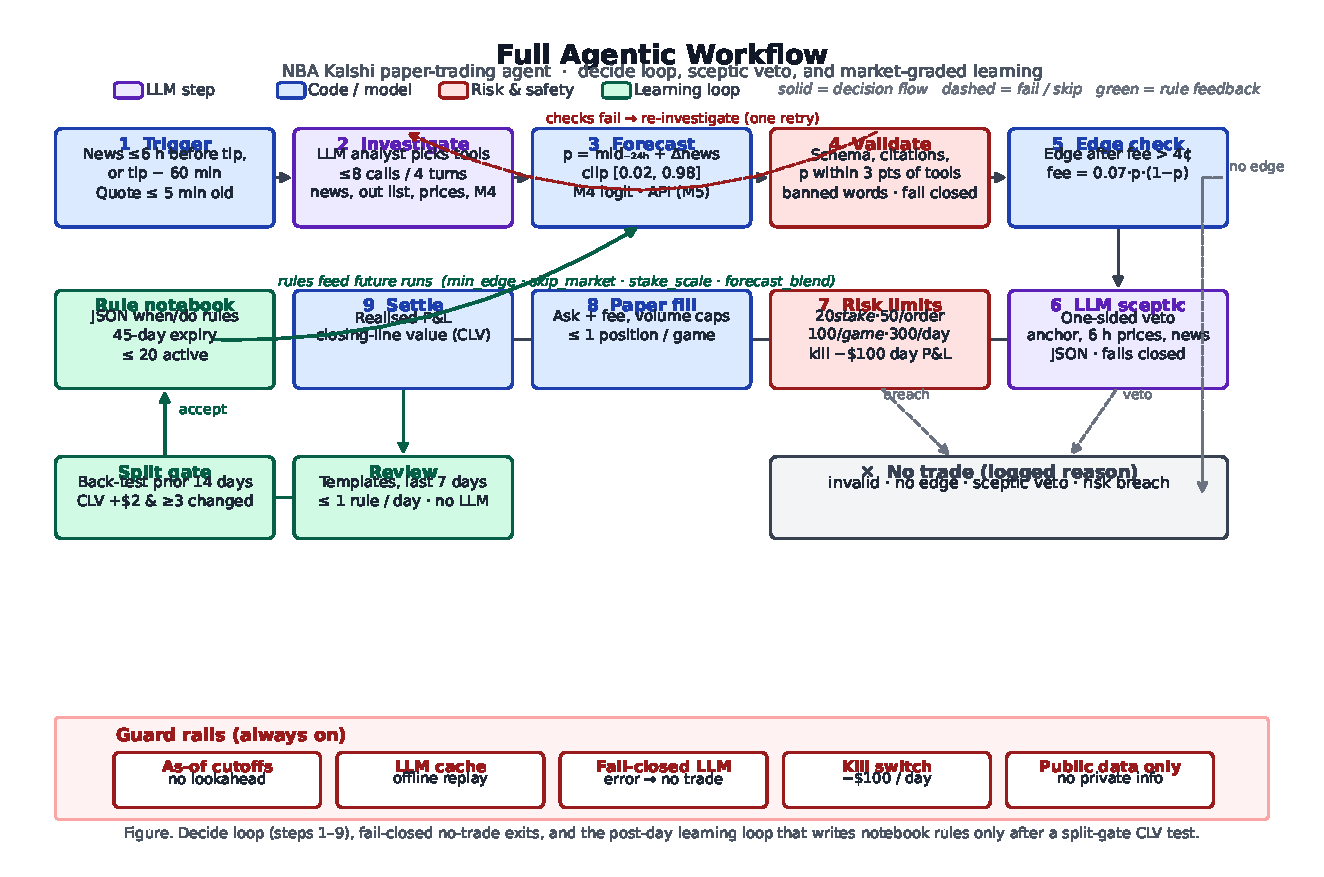
\includegraphics[width=0.72\linewidth]{fig_agentic_workflow.pdf}
\caption{Courtside's backtesting decide loop (MarketAgent / ToolAgent): sceptic
veto, fail paths, and the learning loop. The live desk is the in-game odds product
that this loop is tested against.}
\end{figure}

\subsection{Advantages}
\textbf{Replayability and controlled interpretation.} Timestamped evidence,
forecasts and applied rules are recorded in traces and decision logs. The
as-of contract supports comparisons on the same available information, subject
to the timing assumptions in Section~\ref{sec:methodology}. Numerical checks
constrain LLM errors; passing tests does not establish complete robustness.

\textbf{Bounded tool use.} \code{ToolAgent} may call as-of tools---live quote,
24-hour anchor, public news, M4 win probability and edge helpers---at most
eight times across four turns, then emit a JSON proposal (side, probability,
citations). Code checks the schema, whether citations match the tools, and
whether the stated probability is within three points of a tool-derived
reference. Invalid output becomes a pass. Gemini and DeepSeek backends are
cached so a backtest can be replayed. The live odds desk can show the game
without making that call \cite{llm-evaluation}.

\textbf{The sceptic.} After a buy has already cleared validation and the
fee-adjusted edge rule, an optional sceptic sees a fixed bundle: the proposal,
the code-computed edge, the 24-hour anchor and the move since then, six hours
of prices, the news, and the analyst's tool results. Its prompt asks whether
the market already reflects that information. It returns approve or reject.
Parse errors and banned wording count as a reject, and the reason is kept
short. The sceptic cannot set a new probability or open a trade the code did
not already allow. On the labelled set it kept 8 of 182 proposals
(Dec--Apr CLV \$+7.38) \cite{llm-evaluation}. Later redraws were weaker and
less stable, so that figure is a filter result, not a claim of durable edge.

\textbf{Accountable adaptation.} Nightly proposals cannot activate themselves.
Restricted rule vocabularies, historical gates and expiry constrain adaptation;
split and placebo audits test whether gains reflect better decisions or less
exposure \cite{agentic-rationale,gate-audit}. The gate designs appear in
Section~\ref{subsec:strategy}; empirical gains and uncertainty appear in
Section~\ref{sec:prediction_performance}.

\textbf{Live trading and a logged backtest.} Media and team channels receive
briefs. On the live desk a retail user confirms the in-game stake. In the
backtest a pass is a logged outcome, and the season replay stops new pregame
entries at tip-off. After tip-off the live desk keeps the in-game price and
win chance moving with the game.

% Section 3 integrates the subsequently supplied report.tex contribution.
% Integration edits and factual qualifications are documented in integration_notes.md.
\section{Data and Methodology}
\label{sec:methodology}
\subsection{Data Sources}
Experiments use locally frozen, schema-checked Parquet tables, joining ESPN
schedules and box scores to Kalshi game-winner contracts, prices and settlements.
Table~\ref{tab:data} summarizes the frozen inventory \cite{data-models}.
The 3.9 million price rows are repeated observations; the effective win-model
sample is games, not quote bars.
\begin{table}[h]
\centering\small
\caption{Frozen data inventory and coverage.}
\label{tab:data}
\begin{tabularx}{\linewidth}{L{30mm}Y L{43mm}}
\toprule
Table / source & Coverage and content & Recorded volume\\
\midrule
Games / ESPN & Oct 2023--Jun 2026; schedule and final scores & 3,962 games\\
Player-games / ESPN & Minutes, points, attempts and starts & 85,422 rows; 811 players\\
News / ESPN inactive & Oct 2023--May 2026; availability and reasons & 3,371 items; 1,772 games\\
Markets / Kalshi & Oct 2025--Jun 2026; NBA game winners & 2,632 contracts; 1,316 games\\
Prices / Kalshi & One-minute bid, ask and volume observations & 3,938,368 quote rows\\
Settlements / Kalshi & Binary contract outcomes & 2,634 contracts\\
\bottomrule
\end{tabularx}
\end{table}

Two settled contracts lack matching ESPN games and are excluded from matched
trading evaluation. Market candles cover the 30 hours before contract close;
each candle becomes visible only at its minute-end timestamp. ESPN provides
three seasons of statistics as a practical fallback when NBA endpoints are
inaccessible. Historical news uses inactive lists with a reconstructed
$T-30$-minute timestamp, not an observed publication time. This proxy cannot
establish actual news-arrival latency or a universal direction of bias.

Live adapters separately retrieve official injury reports, ESPN/CBS feeds and
configured Shams, team and reporter accounts, recording provenance and applying
source priority. Polymarket Gamma/CLOB clients provide read-only demo references.
Historical Polymarket trades are not a recorded order book; any reconstructed
spread is an assumption \cite{adapter,implementation}.

\subsection{Data Preprocessing and Feature Engineering}
Seven research tables share schemas, identifiers and UTC timestamps. The
replay's read-only \code{AsOf} view hides unfinished outcomes, unpublished
news and future candles. Quotes used in a decision are at most five minutes
old. Development precedes 1 February 2026. The matched market test is 501
games through 12 April, and 87 later priced games are the holdout. Training
absences come from box scores, while a live override can use only a report
that has already been published \cite{data-models,walkforward}.

\subsection{Prediction Models}
M1 is the rolling and gradient-boosting baseline. M2 is a GRU for points and
minutes. M3 is logistic regression for whether a player plays. M4, the model
on the trading path, is logistic regression on six home-minus-away features:
weighted margin, recent margin, rest, back-to-backs, missing minutes and
missing points. M5 is the shared forecast interface. A neural M4 and a
quote-sequence M6 were tried and did not beat these simpler models, or a
zero-move benchmark, by enough to clear the spread and the fee
\cite{data-models,neural-audit}.

The live desk's in-game win chance is a diffusion update ($\sigma=14$) from
the pre-tip probability, the score and the clock \cite{implementation}. That
update was not fitted on the season sample, and the backtest in
Section~\ref{sec:agent_pnl} uses the pregame anchor and the M4 news shift.

\subsection{Trading Strategy}
\label{subsec:strategy}
At each pregame trigger the research policy anchors to the midpoint 24 hours
before tip (or its earliest available quote), adding M4's news shift:
\begin{equation}
\widehat p=\operatorname{clip}_{[0.02,0.98]}
\big(q_{-24h}+p_{\mathrm{M4,after}}-p_{\mathrm{M4,before}}\big).
\label{eq:anchor}
\end{equation}
For YES, $p_s=\widehat p$ and $c_s=\mathrm{ask}$; for NO,
$p_s=1-\widehat p$ and $c_s=1-\mathrm{bid}$. A candidate requires
$p_s-c_s-0.07c_s(1-c_s)>0.04$. Screening uses the continuous fee approximation;
settlement rounds the aggregate fill fee up to cents. Default stakes are \$20;
optional quarter-Kelly sizing uses a fixed \$1,000 bankroll. Only one position
is held per game. Fresh pre-tip fills are limited to 10\% of recent volume
(or a 200-contract fallback when volume is missing).

Code enforces \$50/order, \$100/game and \$300/day caps, citations and channel
permissions. A \$100 realized-loss stop is configurable; headline reproduction
runs did not enforce it. The nightly reviewer proposes at most one restricted
skip/edge/stake rule. Legacy gates require 0.005 mean-CLV improvement on at
least three changed trades; split gates separate seven selection days from
14 earlier evaluation days and require \$2 total-CLV improvement. Accepted
rules expire after 45 days \cite{gate-audit}.

Settlement records fee-adjusted P\&L and CLV (closing midpoint minus entry).
Brier/log loss grade probabilities; pinball loss and coverage grade quantiles.
Intervals resample game-days, using 2,000 replicates for the reported model
comparisons. Section~\ref{sec:inplay_case_study} is the same product in the
game: a five-point in-game edge and one contract. The season figures are the
backtest; the live desk is where the user confirms an in-game trade.

\section{Implementation and User Workflow}
\label{sec:implementation}
Courtside is the product. Start it with
\texttt{python -m agents.dashboard\_server}.
Three tabs open: Demo, Live data, and Trading tests. Demo and Live data are
the in-game odds desk. Trading tests is the agentic backtest of those trades.

\textbf{Live odds for in-game trading.} Demo and Live data share the match
page. A pregame controller and an in-play controller keep their own state, so
the page can follow one game from the listing through tip-off and the
quarters. The latest valid pre-tip probability starts the live view. After
tip-off the win chance updates from the score, the clock and availability,
and the page sets that chance against the live reference price
\cite{implementation}. Fixtures follow the current NBA date in Eastern Time.
The page shows fair odds, Polymarket references and news
\cite{polymarket,adapter,courtside}. For probability $p$, all-in
decimal odds $D$ and stake $S$, the desk computes
\begin{equation}
 D_{\mathrm{fair}}=\frac{1}{p},\qquad
 p_{\mathrm{break-even}}=\frac{1}{D},\qquad
 \mathbb{E}[\text{net profit}]=S(pD-1).
 \label{eq:selection-value}
\end{equation}
Analysis accounts for depth, estimated fees and a cost buffer. Missing, closed
or stale references block assessment.

On the live slip, Conservative, Balanced and Aggressive are the in-game
acceptance settings: at least 60\% estimated chance and more than four points
of price edge, 45\% and two points, and 25\% and 0.5 points. Negative expected
value passes none. The user keeps the stake. Parlays are a slip feature, not
part of the backtest. The user confirms the trade on the desk.

\textbf{Agentic backtest.} Trading tests is the third tab, and it is the
backtester on the same desk. It archives how the agent decides---the decide
path, the frozen sceptic (8 of 182, Dec--Apr CLV \$+7.38), the walk-forward
P\&L, and the later checks---and then runs one paper trade from the published
rule. The form takes an edge gap (default 4\textcent), a stake (default \$20),
a home-win probability in $[0.02,0.98]$, and an ask. The edge is
$p-\mathrm{ask}-0.07\,\mathrm{ask}(1-\mathrm{ask})$. The desk shows a paper
fill when that edge, in cents, is strictly above the gap, and a pass
otherwise. A fill is clamped at \$50. The \$100/game and \$300/day caps are
part of the backtest policy and are shown on the tab. This run uses the
published edge rule on the numbers the user enters, so a single form does not
place a season replay or a live sceptic call.
\label{sec:implementation-end}


\section{Experimental Evaluation and Results}
\subsection{Prediction Model Performance}
\label{sec:prediction_performance}
On held-out games, M2, M3 and M4 each beat their simple baseline: gradient
boosting for points and minutes, last-game playing status, and M4 without
absence features. That is not the comparison that matters for a trade. On
501 matched games from 1 February to 12 April 2026, the Kalshi midpoint at
tip has Brier score 0.1633. M4 with absences known is 0.1827, worse than the
market one hour before tip by 0.0186 (95\% CI 0.0107--0.0271). Adding the M4
news shift to the 24-hour market moves that anchor from 0.1676 to 0.1663,
which does not beat the contemporaneous price \cite{data-models}. The
backtest therefore treats the market as the anchor and M4 as a news
adjustment, not as a forecast that replaces the book.

\subsection{Agent trading results}
\label{sec:agent_pnl}
These dollars are Courtside's agentic backtest on frozen prices. Trading
tests is that backtest on the desk: it shows this comparison and can run one
paper fill from the same rule. The comparison uses the same recorded prices, the same \$20 stake and
the same caps. Never trading is \$0. The full agent anchors on the 24-hour
market, adds the M4 news shift, and applies the fee-adjusted 4\textcent\ rule
plus the learning gate. The no-learning agent keeps that anchor and edge rule
with an empty notebook. The raw model trades M4 with no market anchor and no
agent. Table~\ref{tab:agent_pnl} is the monthly walk-forward from November
through 12 April \cite{walkforward}.

\begin{table}[h]
\centering\small
\caption{Walk-forward P\&L after fees, November--12 April. Intervals are
95\% game-day bootstrap CIs.}
\label{tab:agent_pnl}
\begin{tabularx}{\linewidth}{Yrrrr}
\toprule
Policy & Trades & P\&L after fees & ROI & CLV \$\\
\midrule
Full agent (anchor + learning) & 157 & $-\$25$ [$-569$, $+564$] & $-0.8\%$ & $-44$\\
Agent, anchor, no learning & 276 & $-\$407$ [$-1{,}324$, $+553$] & $-7.5\%$ & $-84$\\
Raw model, no agent & 711 & $-\$2{,}475$ [$-3{,}995$, $-845$] & $-17.6\%$ & $-255$\\
Never trade & 0 & \$0 & -- & 0\\
\bottomrule
\end{tabularx}
\end{table}

Every policy that trades loses money after fees, and every one has negative
closing-line value, so none beats the closing price. The dollar loss shrinks
as the policy trades less. On the same game-days the full agent finishes
\$382 ahead of the no-learning agent (95\% CI $-\$304$ to $+\$1{,}047$) and
\$2,450 ahead of the raw model (95\% CI $+\$854$ to $+\$3{,}984$). That first
gap is the paired learning gain: both agents see the same days, and the
figure is the sum of the daily P\&L differences. Mean CLV per trade does not
move when learning is on (difference $-0.0002$). The extra dollars come from
skipping trades, not from a better fill on the trades that remain. Against
never trading, the full agent's P\&L interval still covers zero, while its
CLV of $-\$44$ does not.

The February--April split used for the original ablations ranks the policies
the same way. The full agent loses \$32 on 74 trades. Turning learning off,
or freezing the development rules, loses \$247 on 129 trades. Dropping the
market anchor, which is also what a plain model does with no agent, loses
\$2,087 on 366 trades. A win-rate placeholder loses \$429 on 246 trades. In
the later 87-game holdout the full agent takes no trades. The no-learning
agent loses \$74 on six trades. The raw model shows $+\$450$ after fees
(95\% CI $-\$55$ to $+\$1{,}171$) with negative CLV, so that profit is not a
close-beating result. The anchor and the reviewer were designed after early
test inspection; walk-forward checks reduce training leakage but cannot undo
that design history.

The LLM policies were scored on a fixed 40\% subsample of the February--April
decision points, so their dollar totals are not on the same scale as
Table~\ref{tab:agent_pnl} \cite{llm-evaluation}. On that subsample the
deterministic anchor loses \$236 (53 trades). With DeepSeek thinking on, a
one-call LLM makes five trades for $+\$4$; the tool agent without a sceptic
makes 42 trades and loses \$93; with the sceptic it keeps two trades for
$+\$100$ (95\% CI $-\$62$ to $+\$363$). The chat model with the sceptic keeps
no trades, which is the never-trade result. Those intervals cover zero, or
rest on two trades. Results are from saved artifacts, not rerun experiments.

\subsection{Attempts to Improve the Agentic Framework}
Several checks were run after the submission freeze as robustness, not as a
replacement for the frozen headline. On that headline the sceptic kept 8 of
182 validated proposals (Dec--Apr CLV \$+7.38; four paper trades in the
Feb--Apr window). The walk-forward comparison above is unchanged.
Table~\ref{tab:attempts} records the later attempts; none created a reliable
edge.

\begin{table}[h]
\centering\small
\caption{Post-freeze attempts to improve the agent, and their outcomes.}
\label{tab:attempts}
\begin{tabularx}{\linewidth}{L{40mm}Y}
\toprule
Attempt & Outcome\\
\midrule
Sceptic redraws and a softer prompt & Mean CLV about \$+3.27, Fleiss
$\kappa\approx 0.15$. A balanced prompt had AUC $\approx 0.53$. The published
\$+7.38 was an unstable draw.\\
Majority of five calls & Agreement rose ($\kappa\approx 0.39$), but only two
trades were kept (CLV \$+0.83). None of the original eight approvals survived.\\
LLM win probability & Correlation with the live mid $\approx 1$: the model
echoed the price.\\
Other filters & A learned filter, a 1--2\textcent\ pre-filter, and using M4 as
the anchor instead of the market all failed or were left off. Injury timing
was about $-1.4$\textcent\ and trade timing about $-2$\textcent\ after costs.\\
Perfect CLV filter & An after-the-fact ceiling on the same 182 proposals: 55
trades, about \$+39.87 ($\sim$3.6\% on stakes).\\
\bottomrule
\end{tabularx}
\end{table}

The perfect-filter row is an upper bound on redesigning the sceptic for this
market, not a rule that can be traded: it keeps winners after the fact.
These checks support gated abstention, not a durable edge on NBA game-winner
contracts after fees.

\subsection{Case Study: In-Play Market Comparison and Trading Simulation}
\label{sec:inplay_case_study}
The in-game half of Courtside is shown on Sacramento at Orlando, 26 March
2026 (final 117--121). Figure~\ref{fig:inplay} follows the live-desk win
chance against the Kalshi book and Polymarket trades from the scheduled tip.
At Q4 08:49 and a 95--95 tie, that chance is 64.2\% for Orlando, against
trade prices of 0.7600 and 0.7675. Each in-game strategy buys one contract
at its first five-point edge and holds to settlement \cite{section5-case}.

\begin{figure}[h]
\centering
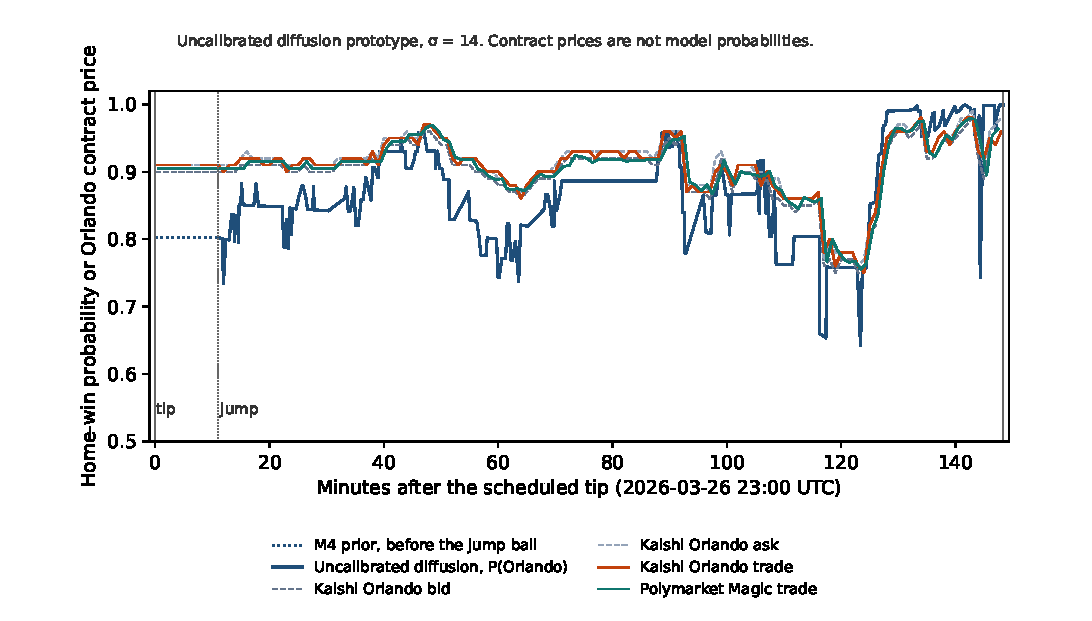
\includegraphics[width=\linewidth]{figure_b_agent_vs_market.pdf}
\caption{Live in-game trading on Orlando, 26 March 2026. The diffusion update
($\sigma=14$) is the desk's win chance. Kalshi bid, ask and trades, and
Polymarket trades, are the live odds. Contract prices are not model probabilities.}
\label{fig:inplay}
\end{figure}

\begin{table}[h]
\centering\small
\caption{Single-game simulation, after the assumed fee.}
\label{tab:inplay_trading}
\begin{tabular}{llrrr}
\toprule
Strategy & Position & Entry quote & Net P\&L & Net ROI\\
\midrule
YES-only & Orlando YES & \$0.84 & $+\$0.15$ & $+17.65\%$\\
NO-only & Orlando NO & \$0.10 & $-\$0.11$ & $-100\%$\\
Two-sided & Orlando NO & \$0.10 & $-\$0.11$ & $-100\%$\\
\bottomrule
\end{tabular}
\end{table}

The two-sided policy enters NO because its prior sits below the market, and
its one-trade limit blocks a later YES. This is one in-game trading path on
the live desk, settled on the recorded prices \cite{section5-case}.

\section{Limitations}
The replay stamps ESPN inactive lists 30 minutes before tip, and on 193 test
games most of the price move in the M4-news direction is already in the book
by then \cite{injury-timing,fairness}. Box-score absences are not prospective
reports. The market beats the model on matched games, and spreads, fees and
delay can erase an apparent edge. Learning cuts the number of trades rather
than the closing-line value of each one. There is no durable edge after
costs, and the single-game chart is one recorded path, not an executable
return. A user study of whether the desk is faster to read is still open.

\section*{Contribution statement}
\begin{center}\small
\begin{tabular}{lr}
\toprule
Name & Factor\\
\midrule
Wu Yaqi & 100\%\\
Wang Yisong & 100\%\\
Zhou Yuanxiang & 100\%\\
Li Yifei & 100\%\\
Ngan Tsz Sui & 100\%\\
Yang Qianlang & 100\%\\
Li Lanqiao & 100\%\\
Fu Yuxuan & 100\%\\
Shen Shangyi & 100\%\\
Zhang Muqun & 100\%\\
Wang Chenghan & 65\%\\
\bottomrule
\end{tabular}
\end{center}

\section*{LLM usage}
The ToolAgent and sceptic sections use Gemini and DeepSeek to propose trades
and to veto an apparent edge. Code validates the schema, the citations and
the probability, and fail-closes: a bad reply becomes a pass. An LLM drafted
and edited the prose of this report, including grammar, across the report.
All prices, fills, caps and statistics come from saved evaluation artifacts,
not from the model.
\label{lastbodypage}

\clearpage
\fancyhead[R]{\small References}
\phantomsection
\addcontentsline{toc}{section}{References}
{\small\raggedright
\begin{thebibliography}{99}
\setlength{\itemsep}{5pt}
\bibitem{wolfers}
J. Wolfers and E. Zitzewitz. Prediction Markets.
\emph{Journal of Economic Perspectives}, 18(2), 107--126, 2004.
\url{https://doi.org/10.1257/0895330041371321}.

\bibitem{polymarket-prices}
Polymarket. \emph{How Are Prices Calculated?} Help Center, 13 March 2026,
accessed 16 October 2026.
\url{https://help.polymarket.com/en/articles/13364488-how-are-prices-calculated}.

\bibitem{aga-2025}
American Gaming Association. \emph{Commercial Gaming Revenue Hits \$78.7
Billion in 2025, Driving Record \$18.1 Billion in Gaming Taxes Nationwide}.
Press release, 26 February 2026, accessed 16 October 2026.
\url{https://americangaming.org/commercial-gaming-revenue-hits-78-7-billion-in-2025-driving-record-18-1-billion-in-gaming-taxes-nationwide/}.

\bibitem{pew-volume}
K.~Radde. \emph{Prediction Markets' Trading Volume Doubled between May and
July, Largely Driven by Sports}. Pew Research Center, 23 September 2026,
accessed 16 October 2026. Notional taker volume from The Block; each contract
is counted at its \$1 payout.
\url{https://www.pewresearch.org/short-reads/2026/09/23/prediction-markets-trading-volume-doubled-between-may-and-july-largely-driven-by-sports/}.

\bibitem{project-readme}
DASC7606C Group 12. \emph{Market-Graded Learning for NBA Game-Impact
Intelligence}. Project README and supplied local working tree, inspected
16 October 2026. \url{https://github.com/Michaelyzr/nba-agent/}.

\bibitem{langgraph}
LangChain. \emph{LangGraph Overview}. Official documentation.
\url{https://docs.langchain.com/oss/python/langgraph/overview}.

\bibitem{react}
S. Yao et al. ReAct: Synergizing Reasoning and Acting in Language Models.
\emph{ICLR}, 2023. \url{https://arxiv.org/abs/2210.03629}.

\bibitem{gate-audit}
DASC7606C Group 12. \emph{Gate Audit}.
\code{evaluation/results/gate_audit.md} and
\code{docs/preregistration_gate.md}. Gate variants, enforcement and
historical-window qualifications.

\bibitem{agentic-rationale}
DASC7606C Group 12. \emph{Why an Agentic Framework}.
\code{docs/why_agentic.md}. Project architecture and empirical rationale.

\bibitem{llm-evaluation}
DASC7606C Group 12. \emph{LLM Tool Agent Evaluation}.
\code{agents/tool_agent.py}, \code{agents/llm_client.py} and
\code{evaluation/results/llm_agent.md}. Optional LLM policies and validation.

\bibitem{walkforward}
DASC7606C Group 12. \emph{Walk-Forward Evaluation, 2025--26 Season}.
\code{evaluation/results/walkforward_summary.md},
\code{significance.md} and \code{holdout.md} in the same directory.

\bibitem{data-models}
DASC7606C Group 12. \emph{Data and Forecast Artifacts}.
\code{evaluation/results/data_overview.csv},
\code{m2_heldout.csv}, \code{m3_heldout.csv}, \code{m4_heldout.csv},
\code{m4_vs_market.csv} and \code{m4_calibration.md} in the same directory;
model implementations in \code{forecast/}.

\bibitem{neural-audit}
DASC7606C Group 12. \emph{Neural Win Models and Market-Impact Robustness}.
\code{evaluation/results/win_nn.md}, \code{m6_robustness.md} and
\code{m6_ablation.md} in the same directory.

\bibitem{implementation}
DASC7606C Group 12. \emph{Courtside Implementation}.
\code{agents/dashboard_server.py}, \code{agents/dashboard_live.py},
\code{agents/pregame.py}, \code{agents/inplay.py}, \code{agents/alerts.py},
\code{agents/bet_review.py} and \code{agents/templates/betting_math.js}.

\bibitem{courtside}
DASC7606C Group 12. \emph{Courtside NBA Betting Desk}.
\code{docs/sample_loop.md}. Current local workflow and risk preferences.

\bibitem{polymarket}
Polymarket Institute. \emph{Making Polymarket Exchange Data Accessible
for Research}. \url{https://institute.polymarket.com/data}.

\bibitem{adapter}
DASC7606C Group 12. \emph{Polymarket NBA Live Data}.
\code{docs/polymarket_live.md}; clients and adapters in \code{data_sources/}.

\bibitem{replaydemo}
DASC7606C Group 12. \emph{January 3, 2024 Injury-Chain Replay}.
\code{docs/samples/injury_chain_2024/report.md},
\code{result.json} and \code{inputs/provenance.json}.

\bibitem{section5-case}
DASC7606C Group 12. \emph{Section 5 Contribution: In-Play Market Comparison
and Trading Simulation}. Supplied
\code{DASC7606C_Group_12_Project_Final_Report_Section5.zip},
including \code{figure_b_agent_vs_market.pdf}, received 16 October 2026.
Summary-level results; the row-level replay ledger was not supplied.

\bibitem{injury-timing}
DASC7606C Group 12. \emph{Price Discovery Against the First Official NBA
Injury Report}. \code{evaluation/results/injury_timing.md}.

\bibitem{fairness}
DASC7606C Group 12. \emph{Consumer Fairness: Evidence from Recorded Kalshi
NBA Game-Winner Prices}.
\code{evaluation/results/consumer_fairness.md}.
\end{thebibliography}
}
\end{document}
